\documentclass[color=green,mathpazo,titlestyle=hang]{elegantbook}

\author{袁勇}
\email{yongyuanstu@gmail.com}
\zhtitle{Python OpenCV}
\zhend{实战}
\entitle{Practical Python and}
\enend{OpenCV}
\version{2.00}
\myquote{一份以示例为驱动介绍图像处理和计算机视觉指南书}
\logo{logo.pdf}
\cover{cover.pdf}

%green color
   \definecolor{main1}{RGB}{0,120,2}
   \definecolor{seco1}{RGB}{230,90,7}
   \definecolor{thid1}{RGB}{0,160,152}
%cyan color
   \definecolor{main2}{RGB}{0,175,152}
   \definecolor{seco2}{RGB}{239,126,30}
   \definecolor{thid2}{RGB}{120,8,13}
%blue color
   \definecolor{main3}{RGB}{20,50,104}
   \definecolor{seco3}{RGB}{180,50,131}
   \definecolor{thid3}{RGB}{7,127,128}

\usepackage{makecell}
\usepackage{lipsum}
\usepackage{texnames}
\usepackage{url}

%定义python语法高亮%
%开始%
\usepackage{listings}
\usepackage{color}

\definecolor{mygreen}{rgb}{0,0.6,0}
\definecolor{mygray}{rgb}{0.5,0.5,0.5}
\definecolor{mymauve}{rgb}{0.58,0,0.82}

\lstset{ %
  numbers=left,                    %设置显示行号在左边
  frame=topline,                   %让代码周围显示边框
  backgroundcolor=\color{white},   % choose the background color
  basicstyle=\footnotesize,        % size of fonts used for the code
  breaklines=true,                 % automatic line breaking only at whitespace
  captionpos=b,                    % sets the caption-position to bottom
  commentstyle=\color{mygreen},    % comment style
  escapeinside={\%*}{*)},          % if you want to add LaTeX within your code
  keywordstyle=\color{blue},       % keyword style
  stringstyle=\color{mymauve},     % string literal style
}
%结束%


\begin{document}
\maketitle
\tableofcontents
\mainmatter

\chapter{简介}

计算机视觉的最终目标是要理解图像中的所展现的内容。对于人类而言,理解图像中的内容是极其容易的,但是对计算机而言,该任务却困难重重。

那为什么还要不辞劳苦地去学习计算机视觉呢?

因为图像无处不在!

无论是在你的智能手机上的个人照片,还是Facebook上的公共照片,亦或是YouTube上的视频,相比于过去我们有了更多的图像——并且我们需要方法来对这些图像的内容进行分析、分类,量化。

比如,你最近是否在Facebook上对你自己的或你朋友的照片加过标记?Facebook是怎样知道一幅图像中人脸的位置在哪里的?

Facebook已经在他们的网站上实现了人脸识别算法,那意味着他们不仅可以在一幅图像中找到人脸,而且他们还可以辨别出这张人脸是谁的。人脸识别技术是计算机视觉在真实世界里的一个应用。

在计算机视觉中还有没有其他类型的有用的应用呢?

当然有,我们可以利用公共图像资源库如Flickr创建我们的三维世界表示。我们可以下载由市民用他们的智能手机和照相机拍摄的成千上万的曼哈顿照片,然后对它们进行分析,并对它们进行组织来构建曼哈顿城市的三维表示,我们还可以通过我们的计算机进行该城市的可视化导航。这听起来是不是很酷?

计算机视觉另一个很火的应用是监控。

虽然监控往往有各种各样的负面含义,但是监控类型还是各有差异的。其中一类监控涉及到视频安全分析,比如抢劫后寻找可能的犯罪嫌疑人。

不过还有另一类型的在零售商店的监控。百货公司可以使用校准后的照相机来跟踪你怎么走过他们的商店,并且在哪些货架子你停下了。

你上一次去最喜欢的服装店时,你有没有在一件春天的最新潮流的牛仔裤前顿足?你在看那条牛仔裤时看了多久?你在看这些牛仔裤时的面部表情是怎样的?你有没有挑出来一条在试衣间里试穿它?所有这些类型的问题计算机视觉监控系统是能够回答的。

计算机视觉还可以应用于医学领域。一年前,我咨询了美国国家癌症研究所,该研究所研发出来了为发现癌症危险因素而能对乳腺癌组织图像进行自动分析。通常,类似这样的任务需要一个多年训练有素的病理学家—并且这将是非常耗时的!

我们的研究证明了计算机视觉可以应用于这些图像,并且能够自动的分析、量化这些细胞结构—没有人工交互!现在,我们分析乳腺组织学图像为癌症的危险因素比以往要快得多了。

当然,计算机视觉还可以用于其他的医学领域,可以用计算机视觉算法分析X-射线,MRI扫描图像以及细胞结构。

你可能听说过的最成功的计算机视觉的成功故事是X-Box 360 Kinect。Kinect用立体相机来理解图像的深度,使得它能够分辨出人类的姿势,当然,这必须得借助一些机器学习的东西。

上面列举的计算机视觉应用并不止于此。

现在计算机视觉在你生活的许多领域盛行,不管你有没有意识到它。我们用计算机视觉算法来分析电影,足球赛,手势识别(手语),车牌(比如你开车开得很快),医学,手术,军事,零售。

我们甚至可以将计算机视觉用于航天。

\chapter{Python及需要的安装包}

要探索计算机视觉世界,首先我们需要安装一些安装包。作为探索计算机视觉之旅的起始,要安装这些安装包特别是OpenCV是非常冗余乏味的,它依赖于你所使用的操作系统。我已经试着将这些安装说明简化成了一份简短的使用指南,不过,正如你所了解的,锁着项目、网站的改变,这些安装说明是会变化的!如果你在安装中遇到了问题,确保查看安装包的网站以获得最新安装说明。

我强力推荐你要么用easy\_install或pip来管理你那些安装包。它会使你的生活变得更简单!

最后,如果你不想自己逐一安装这些安装包的话,我已经预先安装好后所有需要的安装包,并把它们放在一个Ubuntu的虚拟机里。使用该虚拟机可以使你跳过那些繁琐的安装包的安装,直接进入本书的实例中,而不必理会这些安装包的管理、安装说明以及编译错误。

要想获得更多这个预先配置好的虚拟机,可以前往\url{http://www.pyimagesearch.com/practical-python-opencv/}查看详细信息。

现在,让我们来安装这些安装包!

\section{NumPy和SciPy}

NumPy是一个用于Python编程语言的库,它对大型多维数组提供支持。为什么NumPy很重要呢?原因是使用NumPy,我们可以将图像表示为一个多维数组。将图像表示为NumPy数组,不仅易于计算和资源得以有效利用,而且一些其他的图像处理操作和机器学习库也是用NumPy数组来表示的。此外,使用NumPy内置的高水准数学函数,我们能在一幅图像上做快速数值分析。

与NumPy形影不离的是SciPy。SciPy为科学和技术计算提供了更多的支持。

\subsection{Windows}

到目前为止,在你的Windows系统上安装NumPy和SciPy最简单的方式是\url{http://www.scipy.org/install.html}下载并安装二进制分发包。

\subsection{OSX}

如果你运行的是OSX 10.7.0(Lion)或更高版本,NumPy和SciPy已经预先安装好了。

不过,我喜欢安装ScipySuperpack。它包含了最新版的NumPy、SciPy、Matplotlib和其他非常有用的安装包,比如ipython、pandas和scikit-learn。所有的这些安装包是值得安装的,并且如果你在\url{www.PyImageSearch.com}上阅读我的博客,你会发现这些安装包我用得非常的频繁。

\subsection{Linux}

很多Linux发行版,比如Ubuntu,都预先安装有NumPy并且已经是配置好了的。

如果你想要最新版的NumPy和SciPy,你可以从源代码进行编译,不过最简单的方法还是用一个包管理器,比如在Ubuntu上用apt-get。

\section{Matplotlib}

用一句简洁的话概括,matplotlib是一个绘图库。如果你以前用过MATLAB,在matplotlib环境里你很可能会觉得非常的舒适。在分析图像的时候,我们会用到它。不管是画图像直方图还是只是简单地查看图像本身,matplotlib是一个非常有用的工具,你值得将它纳入到你的工具箱中。

\subsection{全平台}

Matplotlib可以在\url{http://matplotlib.org/}上下载。如果你已经安装了ScipySuperpack,那么Matplotlib就已经在你的计算机上安装了。你也可以通过easy\_install或pip来安装它。

此外,在matplotlib官网上还提供了Windows的二进制安装文件。

\section{OpenCV}

如果说NumPy的主要目标是用于有效地表示大型多维数组,那么,OpenCV的主要目标便是实时处理图像。该库从1999年发布以来,已随处可见,直到在2009年发布的第2版中我们才看到了它对NumPy的支持。OpenCV这个库本身是用C/C++写的,但在运行该安装包时它提供了Python的绑定。OpenCV是我手下最喜欢的计算机视觉库,在本书中,我们会经常使用它。

OpenCV的安装是常常会变化的。由于这个库是用C/C++写的,所以在编译的时候需要特别的注意,并要确保预先要安装的东西都已安装。由于OpenCV的最新安装说明是经常会改变的,所以在安装OpenCV时要确保自己去查看OpenCV的网站\url{http://opencv.org/}。

\subsection{Windows和linux}

OpenCV文档提供了在Windows和Linux用二进制版本安装OpenCV非常棒的教程,你可以在这里看到它的安装说明:\url{http://docs.opencv.org/doc/tutorials/introduction/table_of_content_introduction/table_of_content_introduction.html#table-of-content-introduction}。

\subsection{OSX}

过去数年,在OSX上安装OpenCV是一件很痛苦的事,幸运的是现在它的安装已变得越来越简单。你需要安装cmake来构建并编译该OpenCV库,你可以从这里下载cmake\href{http://www.cmake.org/cmake/help/install.html}{http://www.cmake.org/cmake/help/install.html}。

安装cmake后,你就可以从SourceForge资源库检查源代码并进行编译。一般情况下,我发觉Guilherme Defreitas关于怎样在OSX上安装OpenCV的说明是非常棒的,并且为OpenCV的学习给出了一个很好的开始。

你可以在这里找到他的说明:\href{http://www.guidefreitas.com/installing-opencv-2-4-2-on-mac-osx-mountain-lionwith-python-support}{http://www.guidefreitas.com/installing-opencv-2-4-2-on-mac-osx-mountain-lionwith-python-support}。

\section{Mahotas}

如OpenCV一样,Mahotas也依赖于NumPy数组。很多在Mahotas中实现的函数都可以在OpenCV中找到,不过在某些情况下,Mahotas接口比OpenCV接口更容易使用,我们将用Mahotas作为OpenCV的补充。

\subsection{全平台}

在不同的平台上安装Mahotas是极其容易的。假设你已经安装了MumPy和SciPy,那么你所有需要做的只是运行pip install mahotas或easy install mahotas。

既然我们已经安装了所有我们需要的安装包,现在就让我们开始探索计算机视觉世界之旅吧!

\subsection{跳过安装}

正如我在前面提到过,安装这些安装包是费时且繁琐的。如果你想跳过上面那些安装过程而直接进入图像处理和计算机视觉世界,我已经打包好了一个预先配置好了的Ubuntu虚拟机,该虚拟机安装好了上面提到的所有安装包。

如果你对该虚拟机感兴趣并且想要下载它的话(它能够节省你很多时间并避免很多麻烦),你可以到这里下载\href{http://www.pyimagesearch.com/practicalpython-opencv/}{http://www.pyimagesearch.com/practicalpython-opencv/}。

\chapter{载入、显示及保存}

这本书的初衷是成为一本实用手册,用于指引怎样用Python和OpenCV来开始计算机视觉编程。本着这样一条信念,那就让我们不要浪费任何时间了。拿起你的键盘开始写些简单的代码,用于从磁盘载入一幅图像,在屏幕上显示它,并将它用不同的格式写入一个文件。在执行该代码的时候,我们的Python脚本应该可以在屏幕上显示我们载入的图像,正如图3.1所示。

首先,我们创建一个名为load\_display\_save.py来包含我们的代码,现在我们可以开始写代码了:

\begin{lstlisting}[language=python]
import argparse
import cv2

ap = argparse.ArgumentParser()
ap.add_argument("-i", "--image", required = True,
	help = "Path to the image")
args = vars(ap.parse_args())
\end{lstlisting}

我们要做的第一件事是导入在这个例子中我们需要的包。我们用了argparse来解析我们的命令行参数。然后,导入cv2 - 这里cv2就是我们的OpenCV库,它包含了我们需要的图像处理函数。

\begin{figure}[!hbtp]
\centering  %使图片居中显示
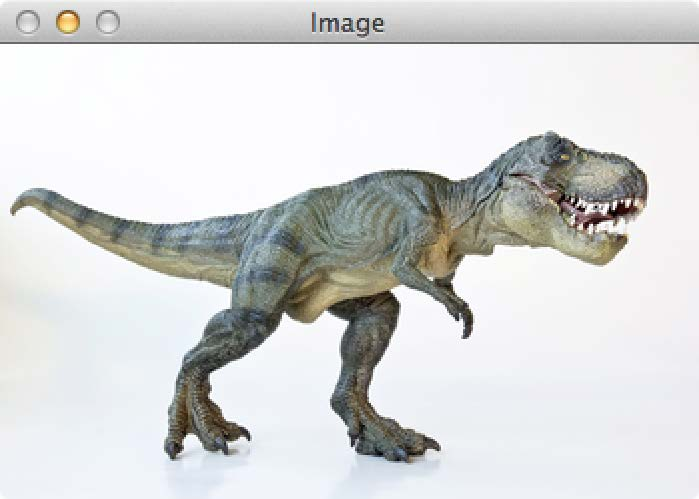
\includegraphics[width=0.8\textwidth]{figure-31.jpg}
\caption{载入并在屏幕上显示一幅霸王龙图像的例子\label{figur:Tyrannosaurus-Rex}}
\end{figure}

上面代码\textbf{第4-7行}用于解析命令行参数。这里我们需要的唯一一个参数是--image:磁盘上图像所在的路径。最后,我们解析这些参数,并在它们保存在一个字典中。

\begin{lstlisting}[language=python]
image = cv2.imread(args["image"])
print "width: %d pixels" % (image.shape[1])
print "height: %d pixels" % (image.shape[0])
print "channels: %d" % (image.shape[2])

cv2.imshow("Image", image)
cv2.waitKey(0)
\end{lstlisting}

既然我们有了图像所在的路径,在\textbf{第8行}我们就可以用cv2.imread函数从磁盘载入该图像。cv2.imread函数返回一个NumPy数组,用于表示一幅图像。

\textbf{第9-11行}检查图像的维数。由于图像是用NumPy数组来表示的,我们可以用shape属性来检查该图像的宽、高,以及颜色通道数。

最后,\textbf{第13行}和\textbf{第14行}用于在屏幕上显示实际载入的图像。cv2.imshow的第一个参数是一个字符串,是窗口的“名字”;第二个参数是我们在\textbf{第8行}从磁盘载入的图像。最后调用了cv2.WaitKey函数来暂停运行的脚本,直到我们在键盘上按下一个键。用参数“0”表示按下任意一个键就会释放暂停。

 我们目前都是学生,接触 \LaTeX{} 的时间也不是很长,因此,对于此模板的错误还请多多包涵! 目前,模板的拓展性或者可移植性有待完善,所以,我们强烈建议用户不要大幅修改模板文件,我们的初衷是提供一套模板,让初学者能够使用一些比较美观,优雅的模板。如果在使用过程中,想修改一些简单的东西需要帮忙,请联系我们,我们的邮箱是:\href{elegantlatex2e@gmail.com}{elegantlatex2e@gmail.com}。我们将竭尽全力提供帮助!

值此版本发行之际,我们 Elegant\LaTeX{} 项目组向大家重新介绍一下我们的工作,我们的主页是 \url{http://elegantlatex.tk},我们这个项目致力于打造一系列美观、优雅、简便的模板方便使用者记录学习历史。其中目前在实施或者在规划中的子项目有 书籍模板ElegantBook、笔记模板ElegantNote、幻灯片模板 ElegantSlide。这些子项目的名词是一体的,请在使用这些名词的时候不要将其断开(如 Elegant Note是不正确的写法)。并且,Elegant\LaTeX{}  Book 指的即是 ElegantBook。

基于本模板追求视觉上的美观的角度,强烈建议使用者安装./fonts/文件夹下的字体。出于版权的考虑,务必不能将此模板用于涉及盈利目的的商业行为,否则,后果自负,本模板带的字体仅供学习使用,如果您喜欢某种字体,请自行购买正版。本文主要使用的字体如下
\begin{itemize}
\itemsep=3pt
\parskip=0pt
\item Adobe Garamond Pro
\item Minion Pro \& Myriad Pro  \& Inconsolata
\item 方正字体
\item 华文中宋
\end{itemize}

\begin{note}
中文正文使用了华文中宋,Minion Pro为英文衬线字体(\verb|\rmfamily|),Myriad Pro为英文非衬线字体(\verb|\sffamily|),Inconsolata 为英文打字机字体(\verb|\ttfamily|)。

并且,如果系统内安装了Adobe 字体,大家可以把模板中使用到的黑体,楷体,宋体等字替换成 Adobe 字体,这样可以达到最佳效果。
\end{note}

本模板基于book文类,所以book的选项对于本模板也是有效的。但是,只支持 \XeLaTeX{},编码为 UTF-8,推荐使用 \TeX{}live编译。作者编写环境为Win8.1(64bit)+\TeX{}live 2013,由于使用了参考文献,所以,编译顺序为\XeLaTeX->\BibTeX->\XeLaTeX->\XeLaTeX。

本文特殊选项设置共有3类,分为{\color{main}颜色} 、{\color{main} 数学字体 }以及{\color{main} 章标题显示风格}。

\chapter{图像基础}

\subsection{那么,什么是像素?}

一般情况下,像素通常采用两种方式进行表示:灰度和彩色。在灰度图像中,每一个像素的像素值在0到255之间,“0”代表“黑色”,“1”表示“白色”。

第一类为{\color{main}颜色}主题设置,内置 3 组颜色主题,分别为 \verb|green|(默认),\verb|cyan|,\verb|blue|,另外还有一个自定义的选项 \verb|nocolor|,用户\textbf{必须}在使用模板的时候选择某个颜色主题或选择 \verb|nocolor|选项。调用颜色主题 \verb|green| 的方法为\verb|\documentclass[green]{elegantbook}|或者使用\verb|\documentclass[color=green]{elegantbook}|。需要改变颜色的话请选择 \verb|nocolor|选项或者使用 \verb|color=none|,然后在导言区定义main、seco、thid颜色,具体的方法如下:
\begin{verbatim}
\definecolor{main}{RGB}{70,70,70}    %定义main颜色值
\definecolor{seco}{RGB}{115,45,2}    %定义seco颜色值
\definecolor{thid}{RGB}{0,80,80}     %定义thid颜色值
\base{blackbase.pdf}                 %可以改为自己想要的图案
\end{verbatim}

第二类为{\color{main}数学字体}设置,有两个可选项,分别是 mathpazo(默认) 和 mtpro2 字体,调用mathpazo 字体使用 \verb|\documentclass[mathpazo]{elegantbook}|,调用 mtpro2 字体时需要把 \verb|mathpazo|换成 \verb|mtpro|,mathpazo 不需要用户自己安装字体,mtpro2 的字体需要自己安装。

\begin{table}[htp]
\centering
\begin{tabular}{ccccc}
\toprule	
	  & green & cyan & blue & 主要使用的环境\\
\midrule
main & \makecell{{\color{main1}\rule{1cm}{1cm}}}& \makecell{{\color{main2}\rule{1cm}{1cm}}}&\makecell{ {\color{main3}\rule{1cm}{1cm}}}& newthem \ newlemma \ newcorol\\

seco &\makecell{ {\color{seco1}\rule{1cm}{1cm}}}& \makecell{{\color{seco2}\rule{1cm}{1cm}}}&\makecell{ {\color{seco3}\rule{1cm}{1cm}}}&newdef\\

thid &\makecell{ {\color{thid1}\rule{1cm}{1cm}}}& \makecell{{\color{thid2}\rule{1cm}{1cm}}}&\makecell{ {\color{thid3}\rule{1cm}{1cm}}}&newprop\\
\bottomrule
\end{tabular}
\caption{ElegantBook 模板中的三套颜色主题\label{tab:color thm}}
\end{table}

第三类为{\color{main} 章标题显示风格},包含 \verb|hang|(默认)与 \verb|display|两种风格,区别在于章标题单行显示(\verb|hang|)与双行显示(\verb|display|),本说明使用了 \verb|hang|。调用方式为 \verb|\documentclass[hang]{elegantbook}|或者 \verb|\documentclass[titlestyle=hang]{elegantbook}|。

综合起来,同时调用三个选项使用 \verb|\documentclass[color=X,Y,titlestyle=Z]{elegantbook}|。其中 \verb|X| 可以选择 \verb|green|,\verb|cyan|,\verb|blue|,\verb|none|;\verb|Y| 可以选择 \verb|mathpazo|或者 \verb|mtpro|;\verb|Z|可以选择 \verb|hang| 或者 \verb|display|。

\subsection{坐标系统概览}
在我们这个模板中,定义了三大类环境
\begin{enumerate}
\item 定理类环境,包含标题和内容两部分。根据格式的不同分为3种
\begin{itemize}
\item {\color{main} newthem、newlemma、newcorol} 环境,颜色为主颜色main,三者编号均以章节为单位;
\item {\color{main} newdef} 环境,含有一个可选项,编号以章节为单位,颜色为seco;
\item {\color{main} newprop} 环境,含有一个可选项,编号以章节为单位,颜色为thid。
\end{itemize}
\item 证明类环境,有  {\color{main} newproof、note、remark、solution} 环境,特点是,有引导符和引导词,并且 newproof、solution 环境有结束标志。
\item 结论类环境,有 {\color{main}  conclusion、assumption、property} 环境,三者均以粗体的引导词为开头,和普通段落格式一致。
\item 示例类环境--- {\color{main} example、exercise}环境,编号以章节为单位,其中exercise环境有引导符。
\item 自定义环境--- {\color{main} custom},带一个必选参数,格式与conclusion 环境很类似。
\end{enumerate}

\subsection{访问和处理像素}
在模板中,可以编辑的字段分别为作者\verb|\author|、\verb|\email|、\verb|\zhtitle|、\verb|\zhend|、\verb|\entitle|、\verb|\enend|、\verb|\version|。并且,可以根据自己的喜好把封面水印效果的\verb|cover.pdf|替换掉,以及封面中用到的\verb|logo.pdf|。

\chapter{画图}

\section{直线和矩形}
\lipsum[3]
考虑如下的随机动态规划问题
\begin{align*}
&\max(\min)\quad \mathbb{E}\int_{t_0}^{t_1}f(t,x,u)\,dt\\
&\quad\mbox{s.t.} \quad dx=g(t,x,u)dt+\sigma(t,x,u)dz\\
&\quad \hspace{2.em} k(0)=k_0\;\text{given}
\end{align*}

where $z$ is stochastic process or white noise or wiener process.

\begin{newdef}[Wiener Process]
If $z$ is wiener process, then for any partition $t_0,t_1,t_2,\ldots$ of time interval, the random variables $z(t_1)-z(t_0),z(t_2)-z(t_1),\ldots$ are independently and normally distributed with zero means and variance $t_1-t_0,t_2-t_1,\ldots$
\end{newdef}

\lipsum[5]

\begin{example}
$E$ and $F$ be two events such that $\mbf{P}(E)=\mbf{P}(F)=1/2$, and $\mbf{P}(E\cap F)=1/3$, let $\mathscr{F}=\sigma(Y)$,  $X$ and $Y$ be the indicate function of $E$ and $F$ respectively. How to compute $\mathbb{E}[ X\mid \mathscr{F} ]$?
\end{example}
\lipsum[4]
\begin{exercise}
let $S=l^\infty=\big\{(x_n)\mid \exists\, M \text{ such that } \forall n, |x_n|\leq M,x_n\in \mathbb{R}\big\}$, $\rho_{\infty}(x,y)=\sup\limits_{n\geq 1}|x_n-y_n|$, show that $\big(l^\infty,\rho_{\infty}\big)$ is complete.
\end{exercise}

\begin{newthem}[勾股定理]
勾股定理的数学表达(Expression)为
\[a^2+b^2=c^2\]
其中$a,b$为直角三角形的两条直角边长,$c$为直角三角形斜边长。
\end{newthem}

\begin{note}
在本模板中,引理(lemma),推论(corollary )的样式和定理的样式一致,包括颜色,仅仅只有计数器的设置不一样。在这个例稿中,我们将不给出引理推论的例子。
\end{note}


\lipsum[4]

\begin{newprop}[最优性原理]
如果$u^*$在$[s,T]$上为最优解,则$u^*$在$[s,T]$任意子区间都是最优解,假设区间为$[t_0,t_1]$的最优解为$u^*$,则$u(t_0)=u^{*}(t_0)$,即初始条件必须还是在$u^*$上。
\end{newprop}

\lipsum[5-6]
\begin{newcorol}
假设$V(\cdot,\cdot)$为值函数,则跟据最大值原理,有如下推论
\[
V(k,z)=\max\Big\{u\big(zf(k)-y\big)+\beta \mathbb{E}V(y,z^\prime)\Big\}
\]
\end{newcorol}

\begin{newproof}
因为 $y^*=\alpha\beta z k^\alpha$,$V(k,z)=\alpha/1-\alpha\beta\ln k_0+1/1-\alpha\beta \ln z_0+\Delta$。
\begin{align*}
\text{右边}&=\Big\{u\big(zf(k)-y\big)+\beta \mathbb{E}V(y,z^\prime)\Big\}\\
&=\ln(zk^\alpha-\alpha\beta zk^\alpha)+\beta\mathbb{E}\Big[\frac{\alpha}{1-\alpha\beta}\ln y+\frac{1}{1-\alpha\beta}\ln z^\prime+\Delta\Big]\\
&=\ln(1-\alpha\beta)zk^\alpha+\beta\Big\{\mathbb{E}\big[\frac{\alpha}{1-\alpha\beta}\ln \alpha\beta z k^\alpha\big]+\frac{1}{1-\alpha\beta}\mathbb{E}[\ln z^\prime]+\Delta\Big\}
\end{align*}
利用$\mathbb{E}[\ln z^\prime]=0$,并将对数展开得
\begin{align*}
\text{右边}&=\ln (1-\alpha\beta)+\ln z+\alpha\ln k+\frac{\alpha\beta}{1-\alpha\beta}\big[\ln \alpha\beta+\ln z+\alpha\ln k\big]+\frac{\beta}{1-\alpha\beta}\mu+\beta \Delta\\
&=\frac{\alpha}{1-\alpha\beta}\ln k+\frac{1}{1-\alpha\beta}\ln z+\Delta
\end{align*}
所以$\text{左边}=\text{右边}$,证毕。
\end{newproof}



\begin{property}
Properties of Cauchy Sequence
\begin{enumerate}\parskip=0pt \itemsep=0pt
\item $\{x_k\}$ is cauchy sequence then $\{x_k^i\}$ is cauchy sequence.
\item $x_k\in \mathbb{R}^n$, $\rho(x,y)$ is Euclidean, then cauchy is equivalent to convergent, $(\mathbb{R}^n,\rho)$ metric space is complete.
\end{enumerate}
\end{property}


\lipsum[7]

\begin{custom}{Application}
This is one example of the custom environment, the key word is given by the option of custom environment.
\end{custom}


\lipsum[6]
\begin{newdef}[Contraction mapping]
$(S,\rho)$ is the metric space, $T: S\to S$, If there exists $\alpha\in(0,1)$ such that for any $x$ and $y\in S$, the distance
\begin{equation}
\rho(Tx,Ty)\leq \alpha\rho(x,y)
\end{equation}
Then $T$ is a {\color{main} contraction mapping}.
\end{newdef}

\begin{remark}
\begin{enumerate}
\parskip=0pt \itemsep=0pt
\item $T:S\to S$, where $S$ is a metric space, if  for any $x,y\in S$, $\rho(Tx,Ty)<\rho(x,y)$ is not contraction mapping.
\item Contraction mapping is continuous map.
\end{enumerate}
\end{remark}


\begin{conclusion}
看到一则小幽默,是这样说的:{\color{main} 别人都关心你飞的有多高,只有我关心你的翅膀好不好吃!}说多了都是泪啊!
\end{conclusion}


\bibliographystyle{ieeetr}
\bibliography{reference}
\addcontentsline{toc}{chapter}{参考文献}

\end{document}
